\setlength{\footskip}{8mm}

\chapter{Methodology}
\label{ch:methodology}

\textit{The different components of the system and how they work together are described in this chapter.}

\section{Hardware}

In the current system, the Mobius Maxi action cam, with fish-eye lens is mounted on  rigid base. The PixHawk 2.4.8 flight controller, having IMU and a GPS module is attached to the rigid base. 


The data from both the devices are fed into a computer with an i7 CPU and 16 GB of RAM running Ubuntu 16.04. The PixHawk 2.4.8 has PX4 as its firmware. Both the devices are connected to the computer through USB interface. In the Mobius cam, auto focus and auto white balance are turned off. 

The test rig is shown in Figure \ref{fig:rigsetup}.

\begin{figure}
	\centering
	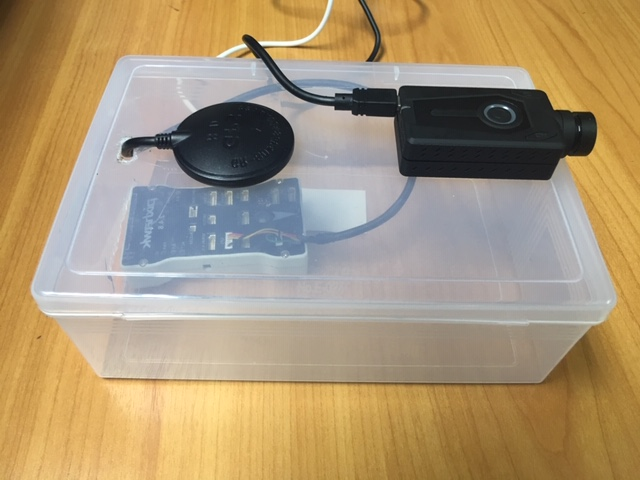
\includegraphics[width=5in]{figures/rig}
	\caption[Close up of the test setup.]{\small 
		Close up of the test setup. }
		\label{fig:rigsetup}
\end{figure}


\section{Software}
Robot Operating System(ROS) Kinetic is running in the test machine. 
The software components are of the test machine are shown in Figure \ref{fig:rosgraph}.

\begin{figure} \label{fig:rosgraph}
	\centering
	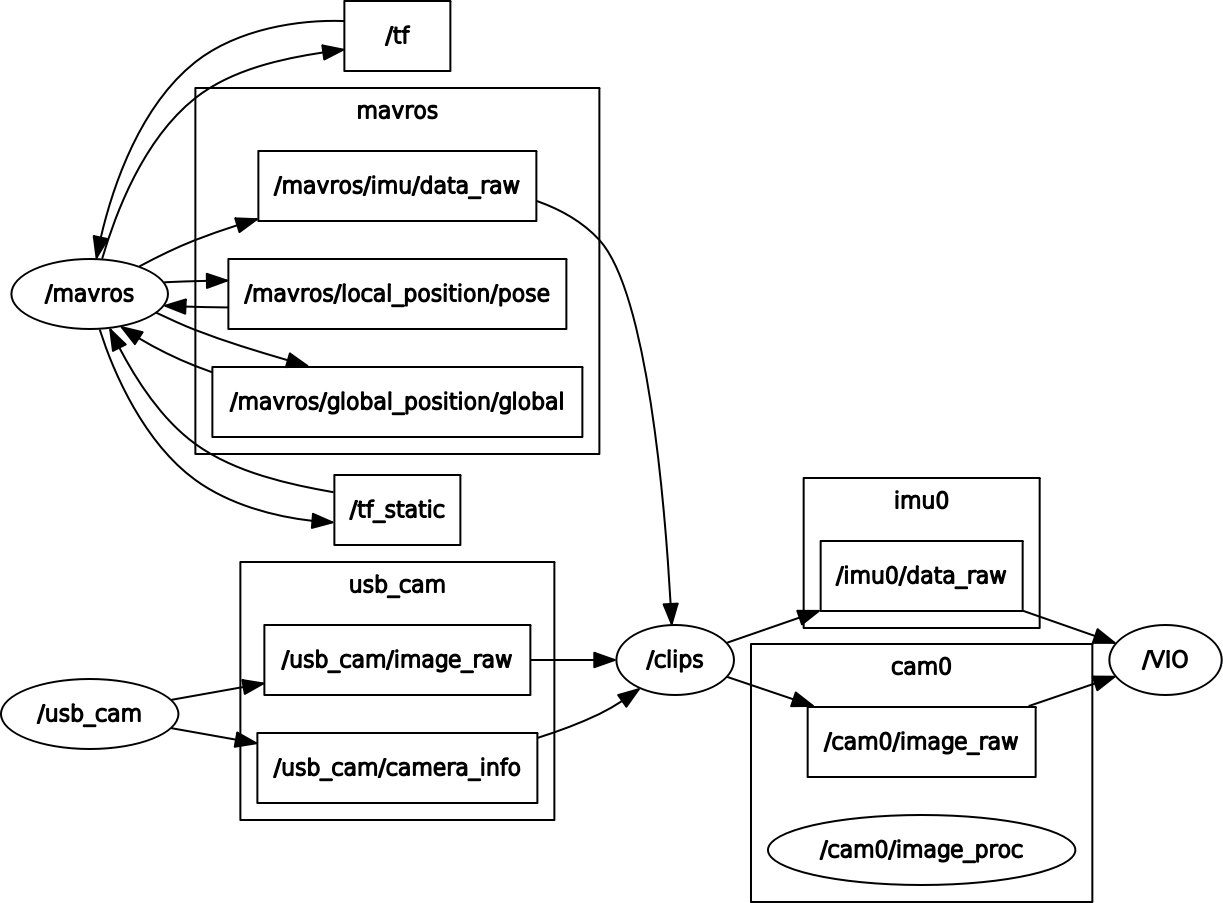
\includegraphics[width=5in]{figures/rosgraph}
	\caption[ROS node tunning on test machine]{\small 
		ROS nodes running on test machine. }
	\label{fig:rig}
\end{figure}

\begin{itemize}
	\item usb\_cam: Modified to support H264 streams.
	\item mavros: Communicates with PixHawk over mavlink protocol.
	\item clips: a custom middleware that ensures there is atleast one IMU data between each image frames
	\item LearnVIORB: Modified to publish pose, point clouds and tf information.
\end{itemize}

\subsection{usb\_cam node}
Mobius Maxi supports H264 hardware encoding. Video stream captured through this H264 stream is more smooth and supports higher framerates. usb\_cam package directly captures video stream from USB cam, however it does not support H264 streams.
The library \textbf{libavutils} which is used by this package does supports H264 streams. I added support for 'h264' in pixel format parameter and a new color format parameter which can accept either 'yuv422p' and 'yuv420p'.
 
\subsection{mavros}
The test machine runs mavros to communicate with PixHawk Flight Controller. 
The PixHawk connection is shown as serial port \textit{/dev/ttyACM0} on the test computer. The baud rate is chosen as \textit{921600}.
PX4 publishes coordinates in NED convention. Mavros automatically converts NED coordinated to ENU coordinates to use with ROS.

Time synchronization between PX4 and ROS is automatically done by \textbf{'sys\_time'} mavros plugin.
A timesync message $M$ is sent at a consistent frequency from the host system to FCU. The host system timestamps the message with the current time $t_s$. The remote system receives it, and adds its timestamp $t_c$ to $M$ and replies back.
The offset between the host system and the remote system is calculated assuming round trip time for the message is equal in both ways.

\begin{equation}
offset = t_s + now - 2t_c
\end{equation}

Sigmoid function is used to interpolate $n$ observations to estimate the time offset. The estimate is further processed with online exponential smoothing filter.
After the estimation has converged, the estimate is used until a maximum number of consecutive observations are received that is higher than a threshold deviation from present estimate. In this case, the estimate is re-calculated with new $n$ observations.

\subsection{clips}
The IMU and camera are independently connected to the test computer and are not tightly bound. Although mavros does time synchronization, there should be some IMU measurement between two different image frames for VIORB to predict the next keyframe location. 
I implemented clips as middleware to ensure that atleast there is one IMU measurement between two image frames.

\subsection{LearnVIORB}
LearnVIORB is a community developed implementation of Visual Inertial ORB SLAM \shortcite{DBLP:journals/corr/Mur-ArtalT16}. This package does not publish pose, and point cloud in real time. I integrated support for publishing pose, point cloud and tf imformation as ros topics. 
I refered to ORB\_SLAM2\_CUDA    \url{https://github.com/hoangthien94/ORB\_SLAM2\_CUDA} which published these topics for implementation.

\subsection{PX4 firmware}
One of the requirements of VIORB is that the IMU measurements should be in hundreds of Hz. PX4 does not natively support more than 50 Hz. Hence to increase it I had to edit \textit{ROMFS/px4fmu\_common/init.d/rcS} file in the source code and recompile the firmware.
rcS file is run at every bootup.

Ardupilot was another option, but it does not support 200 Hz rates.

\begin{lstlisting}
	mavlink stream -d /dev/ttyACM0 -s ATTITUDE -r 200        
	mavlink stream -d /dev/ttyACM0 -s HIGHRES_IMU -r 200
\end{lstlisting}

\section{Calibration}
For a visual inertial SLAM system to work, the following parameters needs to be calibrated beforehand.
 
\subsection{Camera intrinsic parameters}
The camera intrinsic parameters were calibrated with ros camera\_calibration package. This package uses checker board to calculate ${\bf K}$ and the distortion parameters.

\subsection{IMU bias calculation}
Stationary IMU data was recorded for a few hours. Then using \textbf{kalibr\_allan} package allan deviation was calculated and noise density and random walk was derived.

\subsection{Camera IMU tranformation}
VIORB requires ${\bf T}_{CB}$, the camera to IMU transformation. kalibr was used to find the transformation matrix ${\bf T}_{CB}$ and ${\bf T}_{BC}$, where $C$ is the camera's reference frame and $B$ is IMU's reference frame. kalibr uses apriltags or checker board pattern for calibration.

\section{Integration}
A single launch file in clips package starts usb\_cam, mavros, and clips. It publishes \textit{/imu0/data\_raw} and \textit{/cam0/image\_raw}. 

\begin{lstlisting}
<launch>                                                                                                               
	<node name="usb_cam" pkg="usb_cam" 
	type="usb_cam_node" output="screen>                                             
		<param name="video_device" value="/dev/video1" />                                                                  
		<param name="image_width" value="640" />                                                                           
		<param name="image_height" value="480" />                                                                          
		<param name="framerate" value="60" />                                                                              
		<param name="pixel_format" value="h264" />                                                                         
		<param name="color_format" value="yuv420p" />                                                                      
		<param name="camera_frame_id" value="usb_cam" />                                                                   
		<param name="io_method" value="mmap"/>                                                                             
	</node>                                                                                                              
	<include file="$(find mavros)/launch/px4.launch" />                                                                  
	<node name="clips" pkg="clips" 
	type="clips_node" respawn="false" output="screen"/>                                  
	<group ns="cam0">                                                                                                    
		<node name="image_proc" pkg="image_proc"
		type="image_proc" respawn="false" output="screen"/>                       
	</group>                                                                                                             
</launch
\end{lstlisting}

VIORB is launched using another launch file.
\begin{figure}
	\centering
	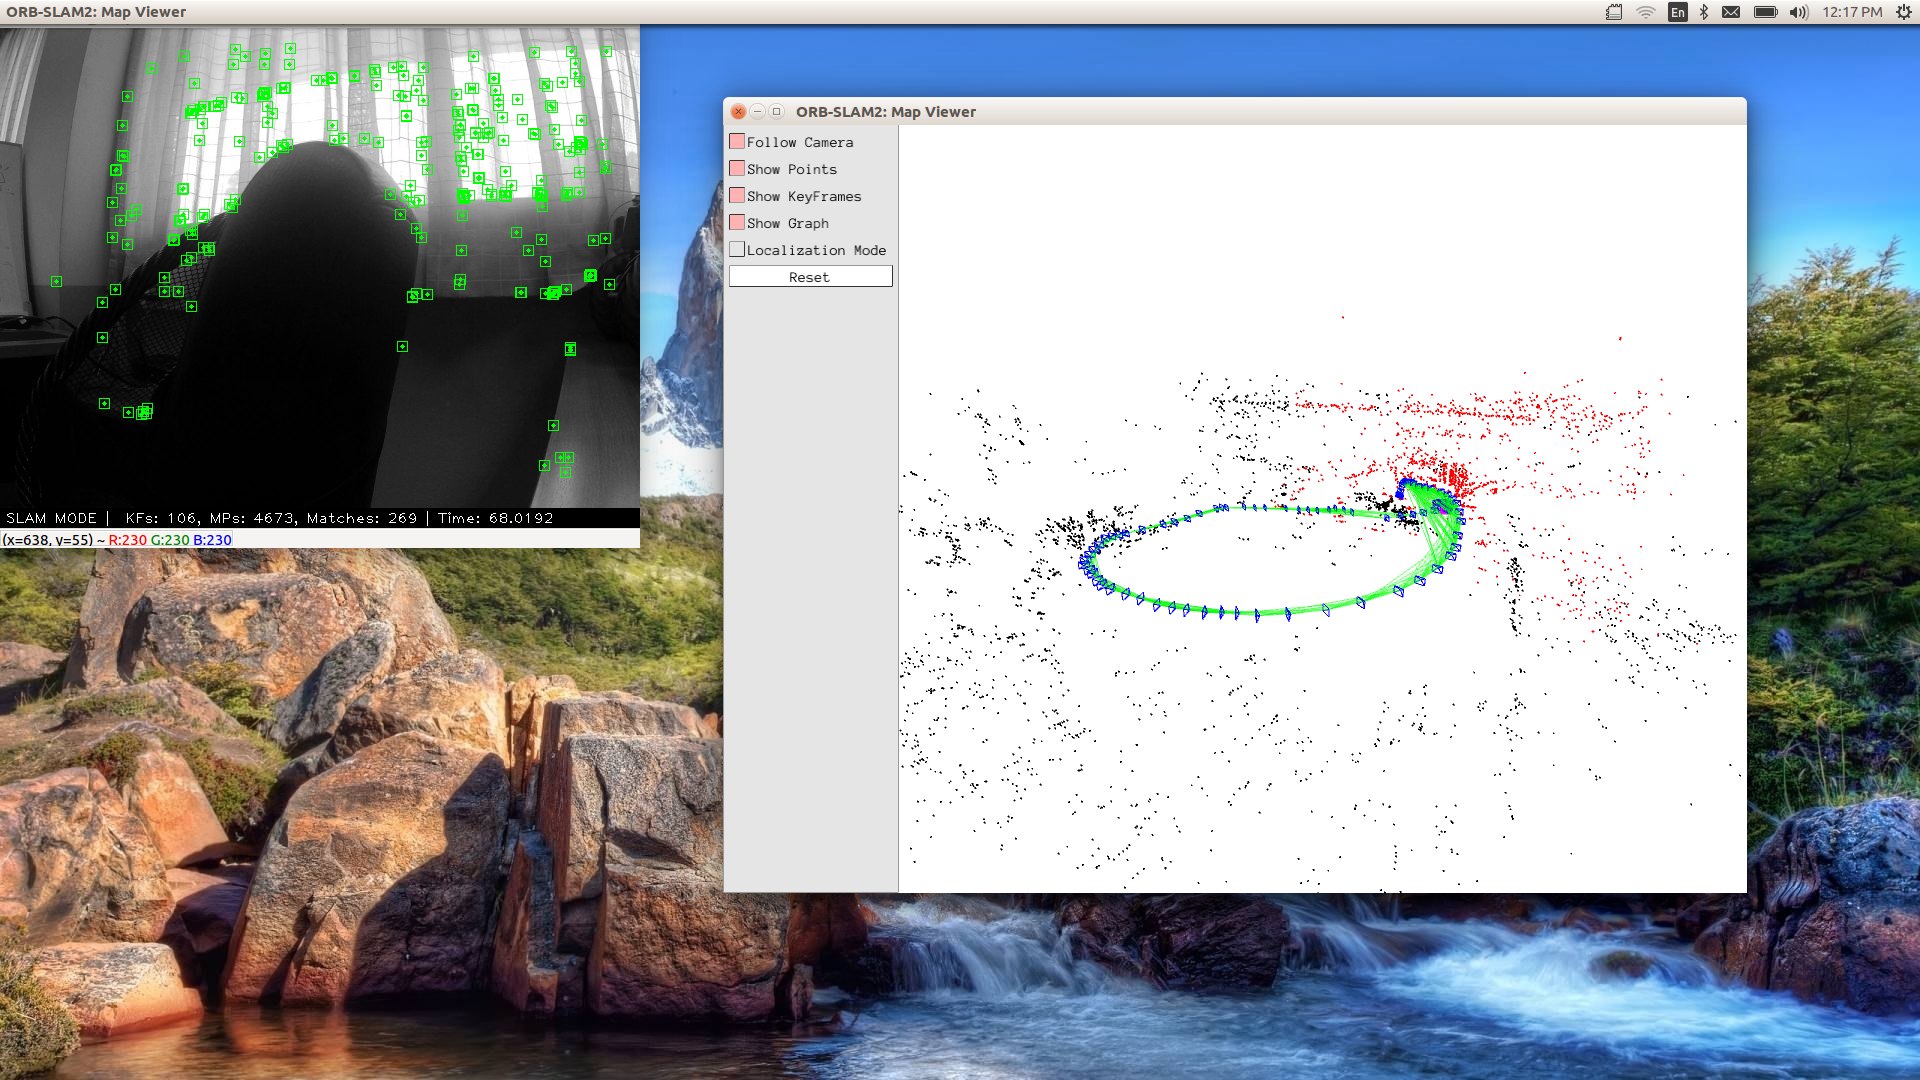
\includegraphics[width=5in]{figures/cloudpoint}
	\caption[Trial run]{\small 
		 A trial run which generates point cloud and pose in CS 203. }
\end{figure}

\FloatBarrier
